\documentclass{article}
\usepackage{arxiv}
\usepackage[utf8]{inputenc} % allow utf-8 input
\usepackage[T1]{fontenc}    % use 8-bit T1 fonts
\usepackage{hyperref}       % hyperlinks
\usepackage{url}            % simple URL typesetting
\usepackage{booktabs}       % professional-quality tables
\usepackage{amsfonts}       % blackboard math symbols
\usepackage{nicefrac}       % compact symbols for 1/2, etc.
\usepackage{microtype}      % microtypography
\usepackage{lipsum}
\usepackage{graphicx}
\usepackage{subcaption}
\usepackage[numbers]{natbib}
\usepackage{float}
\usepackage[nottoc]{tocbibind}

% font size changed from default 10pt to 11pt

\title{A Spatial Analysis of Housing Prices and Supermarket Amenities in London}

\author{
  \large{Kengo Arao}\thanks{With heartfelt thanks to Dr David Candon for dedicated supervision and to Dr Andrei Potlogea for guidance in urban economics}      \thanks{Data and code for this paper are publicly available at \href{https://github.com/KengoA/spatial-analysis-london}{https://github.com/KengoA/spatial-analysis-london}} \\
  Exam Number: B059089 \\
  School of Economics\\
  The University of Edinburgh\\
  \texttt{kengoarao@outlook.com}
}

\begin{document}
\maketitle

\begin{abstract}
Integrating the bid rent theory by Alonso (1964), Muth (1969), and Mills (1972) into the hedonic pricing model by Rosen (1974), I analyse the dynamics of housing prices in Greater London by constructing spatial features from Uber Movement and OpenStreetMap. Estimating the commuting cost to the city centre, I find that the average travelling time on the road in the morning has a larger effect on housing prices than the orthodromic distance, while the latter has a higher explanatory power overall. I then introduce heterogeneity in local amenities by accounting for factors such as supermarkets, land use, food establishments and educational institutions, and find that the presence of high-end supermarkets, private schools, and golf courses are strongly associated with high housing prices, whereas industrial land use, fast food restaurants, and low-end supermarkets show negative correlations. Using planning permissions and mean retail floor spaces as instruments, I provide causal evidence that different classes of supermarkets have opposing effects on housing prices.

\end{abstract}

% keywords can be removed
% \keywords{First keyword \and Second keyword \and More}
\begin{center}
    \textbf{Word Count}: 10,000
\end{center}

\newpage
\tableofcontents

\newpage
\section{Introduction} \label{section:intro}
In every metropolitan area, housing price has a strong influence over individual consumption choices and hence important implications in social mobility and quality of life. In light of the rapid urbanisation with 68\% of the world population expected to live in urban areas by 2050 (United Nations, 2018), the underlying mechanism of urban housing markets has been under heavy scrutiny in the fields of urban research and economic geography, as well as being a focal point of major media outlets in the United Kingdom (The Guardian, 2019). One example of dynamically changing urban landscapes is the penetration of German supermarkets into the British grocery market in recent years (Davey, 2018), with their low-price policies affecting local consumption behaviours. Several newspaper articles popularised the term 'the Waitrose effect' based on a research paper by Lloyds Bank (2016), which states that proximity to a supermarket implies house price premium upwards of 43,000 pound sterling (The Telegraph, 2016; The Independent, 2017). The causal effects of the presence of supermarkets and the importance of other features affecting the housing prices, nonetheless, remain to be understood.
 
This objective of this paper is to investigate the effects of such urban amenities and neighbourhood characteristics on the housing prices at the local level, with the empirical models inspired by the bid rent theory by Alonso (1964) for the commuting cost to the city centre and the hedonic pricing model by Rosen (1974) for product differentiation with objective characteristics. In doing so, I provide novelty in two respects. The first is construction of local amenity variables from OpenStreetMap, an open-sourced collaborative mapping project, which is applicable beyond the scope of the Greater London Area that my empirical analysis is concerned with. The second is the causal analysis of supermarket amenities in relation to housing prices with instrumental variables, in which I demonstrate that the presence of high-end supermarkets such as Waitrose and Marks and Spencer cause higher housing prices, controlling for other local amenities and distance to the Central Business District (CBD).

This paper is structured as follows. Section \ref{section:lit} first provides the theoretical foundations of seminal models by Alonso (1964) and Rosen (1974) and discusses the monocentricity assumption in the literature and in the context of London, and also review research into local amenities that affect housing prices such as education and consumption accessibility. Section \ref{section:data} briefly describes data sources and their properties, followed by Section \ref{section:variables} where I illustrate data transformation and feature engineering methods. Section \ref{section:model} describes regression models and the results in accordance with the theoretical framework, and provide causal analysis with instrumental variables for high-end and low-end supermarkets. Section \ref{section:discussion} discusses limitations and external validity of this study, and Section \ref{section:conclusion} concludes.


\section{Conceptual Frameworks and Literature Review} \label{section:lit}
This section introduces two theories that are fundamental to the empirical models I develop in Section \ref{section:model}. I then review a body of empirical research regarding the monocentricity assumption by Alonso (1964), as well as several heterogeneous urban amenities to reinforce the scopes of variable construction in Section \ref{section:variables}.

\subsection{Bid Rent Theory}
A starting point for understanding urban complexity is a geographic economic theory by Alonso (1964), Muth (1969), and Mills (1972) called bid-rent theory, which refers to the relationship between the distance from the the city centre and real estate price. The basic intuition is that the housing price increases as you move closer towards the CBD, and consumers face a trade-off between housing costs and commuting costs. A simple version of this model described below, the monocentric city model, underpins the empirical specifications throughout this paper and requires the following five assumptions, the first of which will be relaxed in the next section.
\begin{itemize}
\setlength\itemsep{0.1em}
\item Residents are homogeneous and live in a featureless urban area where all the jobs are located in the CBD
\item Each resident is a worker and commutes to a job in the CBD
\item Each worker receives an urban wage $w$ with inelastic labour supply
\item Commuting from distance $d$ entails a linear commuting cost $t(d) = \tau d$
\item Each worker consumes 1 unit of housing which is produced solely  with land
\end{itemize}
Let $p_H (d)$ denote the price of housing located at distance $d$ from the CBD, then a worker's preference can be written as a linear utility function:
\begin{center}
$u = w - p _ { H } ( d ) - t ( d ) = w - p _ { H } ( d ) - \tau d$
\end{center}
With an outside option in the hinterland $\overline{u}$, the spatial equilibrium requires
\begin{center}
$u = w - p _ { H } ( d ) - \tau d = \overline { u }$
\end{center}
Rearranging and partially differentiating $p_H (d)$ with respect to $d$ yields 
\begin{center}
$\frac { \partial p _ { H } ( d ) } { \partial d } = t ^ { \prime } ( d ) = - \tau \quad \forall d \leq \overline { d }$
\end{center}
Let $\overline{d}$ be the upper bound for distance and $\underline{r} > 0$ be the rent for alternative use of land. Then, the equilibrium rent can be written as:

\begin{center}
$p _ { H } ( d ) = \underline { r } + \int _ { d } ^ { \overline { d } } t ^ { \prime } ( \delta ) d \delta = \underline { r } + \tau ( \overline { d } - d )$
\end{center}
Since the alternative land rent $\underline{r}$ is difficult to estimate in practice, I flip the sign of the equation such that 
\begin{center}
$p _ { H } ( d ) = \overline { r } - \int _ { \underline { d } } ^ { d } t ^ { \prime } ( \delta ) d \delta = \overline { r } - \tau ( d - \underline { d } )$
\end{center}
where $\overline{r}$ is the rent in the CBD and $\underline{d}$ is the lower bound for distance, which is 0 at the CBD. This equation hence represents a function of the price of housing which is linearly decreasing in distance from the CBD $d$, which is simply
\begin{center}
$p _ { H } ( d ) = \overline { r } - \tau d$
\end{center}
This will be the basis of the univariate regression models where I estimate the coefficient $\tau$ associated with two measures of distance between the CBD and a given area; orthodromic distance and commuting time cost approximated by Uber Movement Data. $\overline{r}$ is the constant term which represents the rent in the CBD at distance $d = 0$.

\subsection{Heterogeneous Amenities and Hedonic Pricing Model}
In the simple monocentric model, it was assumed that the city is a featureless plane without any urban amenities such as restaurants and cafes. This assumption is now relaxed by introducing heterogeneity in amenities where each subsection of the city has its own characteristics that residents assign specific values to. This is an extension of the hedonic pricing model by Rosen (1974) where a product is valued by its internal characteristics and external factors that are both homogeneous and objective. In Rosen's model, the class of products offers a package of quantifiable characteristics represented by a vector 

\begin{center}
    $z = \left( z _ { 1 } , z _ { 2 } , \dots , z _ { n } \right)$
\end{center}

where $z_i$ is the $i$-th characteristic on a plane of features, which in our case corresponds to the amount of a certain amenity that is present in the neighbourhood. Importantly, market clearing prices $p(z)$ are determined by consumer tastes and production costs, which equalise across buyers and identify the demand structure:

\begin{center}
    $p ( z ) = p \left( z _ { 1 } , z _ { 2 } , \dots , z _ { n } \right)$
\end{center}

The existence of market equilibrium in pure competition and decomposition of products into attributes $z_i$ is the theoretical grounding of the multivariate regressions of this paper, where the first element is the distance from the CBD and $2, 3, ..., n$-th elements are features based on geographical distributions of urban amenities.

This paper confines its scope to sections of London boroughs defined as Middle Layer Super Output Area (MSOA) which was created to provide a statistical overview of the population, with an average of 8346 in 2010 (The Greater London Authority, 2014). While the hedonic pricing model is often applied for a smaller unit of housing such as a house or a flat, Rosen's criterion for objectivity is better suited for neighbourhood characteristics as some factors in a individual housing unit such as architectural styles and view from the window could entail heterogeneous preferences that are prone to subjectivity.

\subsection{Monocentricity Assumption and Current Research on Housing Prices}
Bid rent theory remains heavily influential in empirical investigations in urban economics, and location has been a dominant explanatory factor for housing prices and urban structures. However, the assumption of monocentric cities has been actively contested both in theoretical and empirical terms. Fujita and Ogawa (1982) criticise the exogenous location of the CBD, and provide general equilibrium models where employment centres are endogenously determined by firms and agents.
From an empirical point of view, McMillen (2001) highlights the rise of polycentric city structures in the United States, and identifies employment subcenters in Milwaukee, where employment opportunities are scattered around across the metropolitan area with only 6.7\% of them located in the CBD. A more systematic study is conducted by Arribas-Bel and Sanz-Gracia (2014). They analyse the time trend of high employment density in 359 U.S. metropolitan areas in 1990, 2000, and 2010, and find that employment centres are still largely concentrated centrally, with 57\% of all metropolitan areas exhibiting monocentric structures in 2010. It is noteworthy that there is a large variance in employment share figures in these studies, depending on the definition and scope of the CBD. In general, while there is an increasing number of empirical studies that showcase the polycentric urban structures, the assumption of single-core centres appears to hold across modern metropolitan areas. 

In the context of London, European Commission (1999) describes London as a monocentric city given the strong transport connectivity to the periphery areas and concentration of economic activities in the city. On the other hand, there is limited yet meaningful evidence of the polycentric nature of London. Utilising the large scale data of Oyster card transactions in the London subway, Roth et al. (2011) investigate the individual intraurban flows with the Tube network to identify several basins of attraction in London, the largest of which is West End followed by the City of London area. Importantly, they also demonstrate the significance of the Docklands area where a number of financial firms are located. Similarly, Park (2011) studies commuting flows based on the 2001 Census and Office for National Statistics data, and identifies a cluster of employment in Westminster, Camden and City areas. Despite the evidence of heterogeneity especially within the central London, the monocentric structure seems to be present in the scale of Greater London. Hence, this paper follows Park (2011) and impose Alonso's (1964) original assumption of monocentricity in examining London's urban structure. Identification of the CBD is further explored in Section \ref{subsection:CBD}.

Regarding urban amenities, Niu and Liu (2017) provide several proxies to measure accessibility to key economic activities in modelling urban housing price in Beijing. In addition to the employment centre, they investigate the effects of education, consumption and medical accessibility, and calculate the household demand structure for housing prices. They demonstrate that the employment accessibility has by far the highest importance as an economic activity, followed education and consumption and medical services. While their results are limited in statistical significance and the scope, their findings motivate the construction of measures of consumption accessibility through the number of supermarkets, and education accessibility in the form of private schools in Section \ref{subsection:school}. In relation to education, Department for Education (2017) finds that home prices in England have a price premium near the schools in the top 10 percent in terms of standardised test performance, where house prices are higher by 8.0\% for primary schools and 6.4\% for secondary schools, holding everything constant.

An important aspect of daily consumption accessibility that affects individuals universally across socioeconomic strata is supermarkets. Despite the lack of rigorous academic research specifically into supermarket amenities, Lloyds Bank's (2016) research into the housing premium of different supermarket chains at the post code level was influential in the British media which led to the popularisation of the term "the Waitrose effect" (The Independent, 2017). Supermarkets in general are associated with positive housing price premium in varying degrees, with Waitrose and Sainsbury's having a strong premium of £38,666 and £27,939 on average, followed by Marks and Spencer (£27,1812), Tesco (£22,072), Iceland(£20,034), Coop (£17,904), and Morrisons (£10,558). The lower end of distribution includes discount supermarkets such as Asda, Lidl, and Aldi which have marginal levels of premium at £5,026, £3,926 and £1,333, respectively. This translates into a premium of 10\% for Waitrose and Sainsbury's, while those of Asda, Lidl and Aldi are limited to 1-2\%. However, their method to calculate these figures is deeply problematic, in that they compare the average housing prices between a postcode area where a target supermarket and an area in the same town where it is not. This approach disregards heterogeneity in amenities in different areas and creates a downward bias to areas without any of the target supermarkets, which makes it difficult to isolate the effects of supermarket amenities especially in densely populated areas such as London. Reflecting on this, I will construct a linear model of housing prices controlling for other accessibility measures that affect the housing prices. 


\section{Data} \label{section:data}
\subsection{Geographic Boundaries}
The geographic unit for this paper's analysis is based on output areas (OAs) which have been the basis for UK Census since 2001, and are designed to be homogeneous in terms of population sizes and household characteristics (Office for National Statistics, 2019). For compatibility with the housing prices data, an aggregate measure of Middle Layer Super Output Areas (MSOA) is obtained from London Datastore (201 for the empirical analyses throughout the paper with the population ranging from 5000 to 15000 and number of households from 2000 to 6000, where, in the case of Greater London, there are 984 MSOAs and the average population of 8346 in 2010 (Greater London Authority, 2014).

\subsection{Housing Prices}
Urban rent in each neighbourhood is approximated by property sales registered with Land Registry (2019) which records property sales at the individual dwelling level. This is aggregated for each MSOA at the end of the calendar year for mean and median prices. Table 1 shows descriptive statistics for mean housing prices for each MSOA for the year of 2017, which clearly shows that the prices are not normally distributed with the mean value almost approaching the 75\% percentile, as this is skewed by significantly high housing prices in the central London. Figure 1 maps the geographical distribution of mean housing prices visually both on raw and the log scale.


\begin{table}[H]
\caption{Descriptive Statistics for Mean Housing Prices (GBP)} 
  \label{} 
\begin{tabular}{lrrrrrrrr}
\toprule
{} &  count &       mean &        std &       min &       25\% &       50\% &       75\% &        max \\
\midrule
Value &  983.0 &  603715.49 &  387541.06 &  226536.0 &  391267.0 &  495010.0 &  673064.5 &  4416659.0 \\
\bottomrule
\end{tabular}
\end{table}

\begin{figure}[H]
  \centering
  \begin{subfigure}{.45\textwidth}
      \centering
      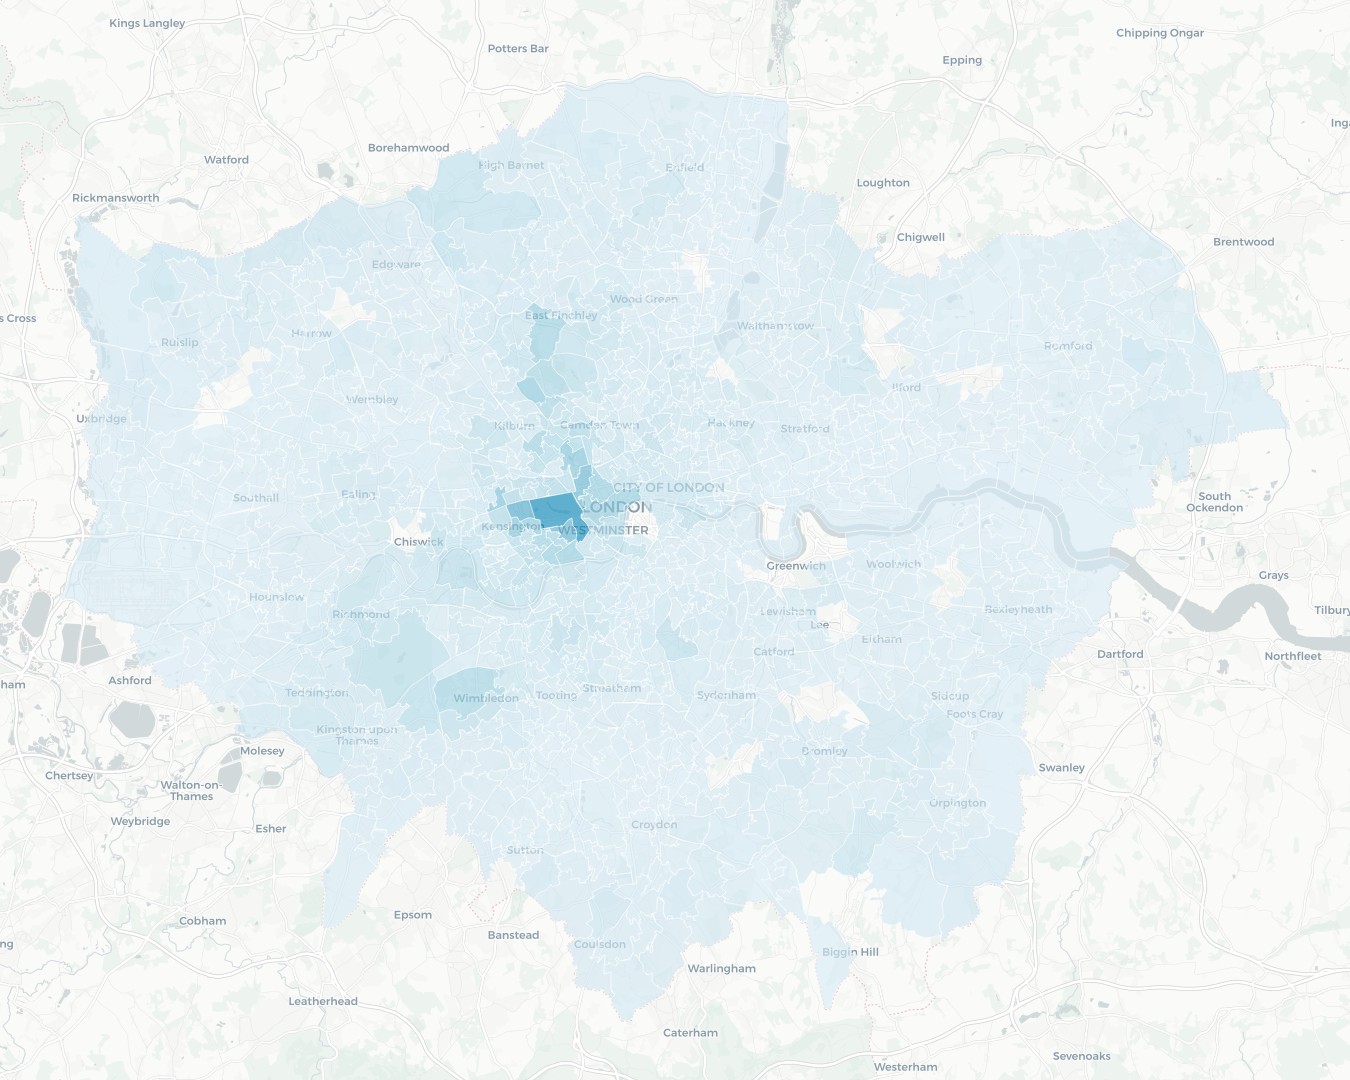
\includegraphics[width=.95\linewidth]{images/housing_raw_mean.png}
      \caption{Mean Housing Price}
      \label{fig:1(a)}
  \end{subfigure}
  \begin{subfigure}{.45\textwidth}
      \centering
      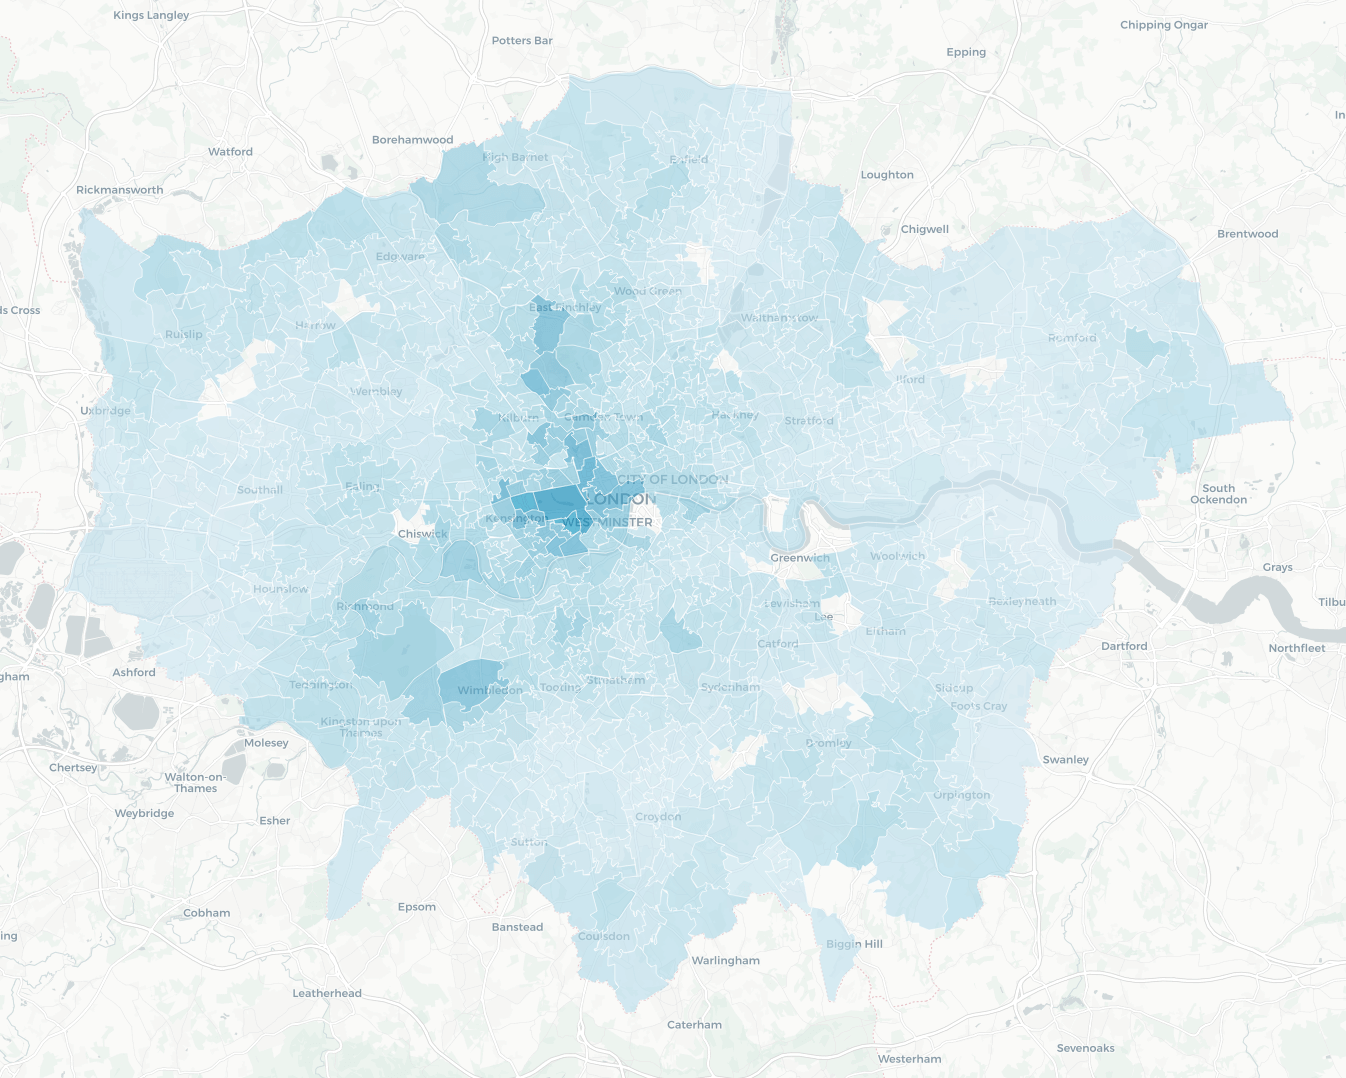
\includegraphics[width=.95\linewidth]{images/housing_log_mean.png}
      \caption{log(Mean Housing Price)}
      \label{fig:1(b)}
  \end{subfigure}
  \caption{Housing Price Distribution Across Greater London}
  \label{fig:price_distribution}
\end{figure}

\subsection{Distance}
Each MSOA is defined as a polygon with edges represented with geographic coordinates (i.e. Trafalgar Square is at 51.5080 N, 0.1281 W), which will be the basis for the geometric distance measure between each MSOA and the CBD in Section \ref{section:variables}. The second distance measure is morning commuting time on the road, which is approximated from Uber Movement data (2019) that provides anonymised travel data in the form of summary statistics such as mean travel times and standard deviation at a given hour of the day. This data covers major cities in North America, Europe, Australia and India where Uber usage is high, and quarterly data is available for London since 2016.

\subsection{Geographical Features}
The central focus of this paper is the use of geographical features from OpenStreetMap, which is a collaborative mapping scheme launched in 2004.


\subsection{Private School Data} \label{subsection:school}
Ndaji et al. (2016) investigate the difference in educational achievements between independent schools and state schools in the United Kingdom, and demonstrate that students in independent schools had better results by 0.64 GCSE grades, controlling for prior academic ability, socioeconomic disadvantages, and gender differences. This discrepancy is equivalent to additional two years of schooling by the age of 16. Hence, I posit that private school is a desirable education amenity that households with children are especially attracted to. As OpenStreetMap does not provide school type in details, I compile an original dataset for private schools in Greater London in a programmatic manner by scraping a web page by Independent Schools Concil (2019), which provides a comprehensive list of private schools in London providing primary and secondary education. Addresses are then converted into longitudes and latitudes using the \texttt{geocoders.Nominatim} module from \texttt{geopy} library in Python, such that each school falls onto one of the MSOAs.

\section{Variable Construction} \label{section:variables}
\subsection{Defining the City Centre}\label{subsection:CBD}
\begin{figure}[H]
  \centering
  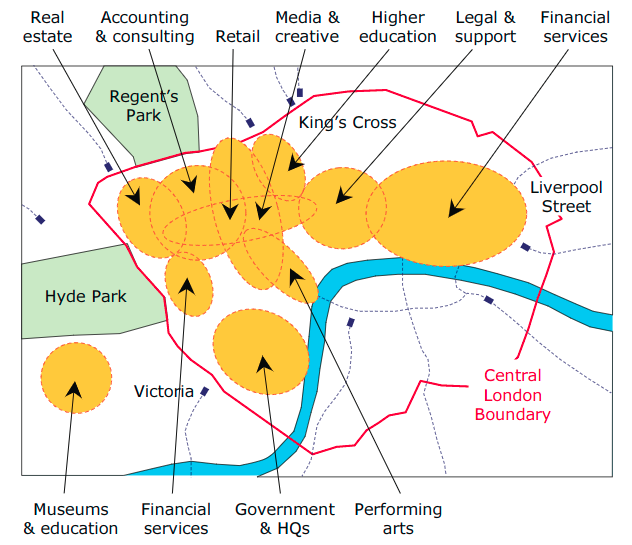
\includegraphics[width=0.5\linewidth]{images/cbd.png}
  \caption{Distribution of CBD functions in London (Greater London Authority, 2008)}
  \label{fig:cbd}
\end{figure}

\begin{figure}[H]
  \centering
  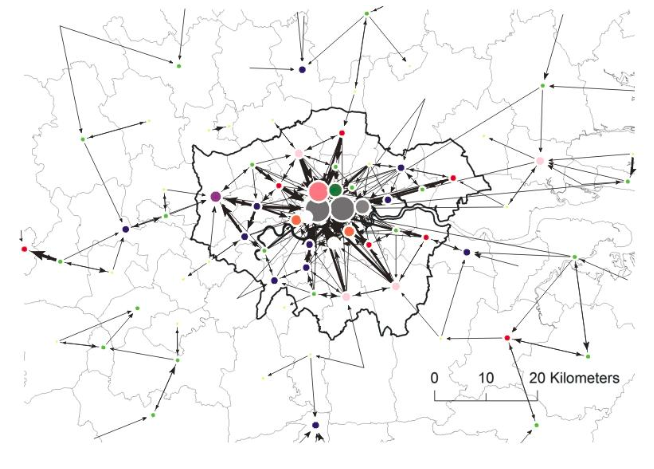
\includegraphics[width=0.5\linewidth]{images/park2011.png}
  \caption{Commute Network into Central London (Park, 2011)}
  \label{fig:cbd}
\end{figure}


Michaels \& Smith (1990) on market segmentation and necessity for multiple price functions -> not truly monocentric - commuting functions


\subsection{Distance Measures}
The following illustrates how two measures of distance are constructed. To ensure an approximately normal distribution, both distance measures are log-transformed in the regression models.
\subsubsection{Orthodromic Distance}
The first measure of distance is the distance between two points on a sphere; the centroid of a given area $C_k$ and the centroid of the CBD, $C_0$, which is then converted to miles for ease of interpretation. Each MSOA is represented by a simple polygon where each vertex consists of longitude and latitude in the standard geographic coordinate system (Bolstad, 2016). Let $v_{i,j}$ be a vertex in a N-gon where $v_i$ is a longitude and $v_j$ is a latitude. Then the centroid for a given $k$ is expressed as 

\begin{center}
    $C_k = (C_{ki}, C_{kj})  = (\frac{1}{n} \Sigma_{i=1}^{N} v_i, \frac{1}{n} \Sigma_{j=1}^{N} v_j) $
\end{center}

where $C_{ki}$ and $C_{kj}$ are longitude and latitude for the centroid, respectively. Since the centroids are relatively close to each other with each located in our setting, the Haversine formula (Van Brummelen, 2017) is used for numerical stability to calculate the distance $d$ between two points on a sphere\footnote{The Haversine formula is computationally better conditioned than the arc length formula when two points are close to each other on the sphere due to rounding errors}, $C_0$ and $C_k$, such that

\begin{center}
    $d =2 r \arcsin \left(\sqrt{\sin ^{2}\left(\frac{C_{0i}-C_{ki}}{2}\right)+\cos \left(C_{ki}\right) \cos \left(C_{0i}\right) \sin ^{2}\left(\frac{C_{0j}-C_{kj}}{2}\right)}\right)$
\end{center}
where $r$ is the radius of earth in a desired unit of length, which in this case miles with $r = 3956$. 

\subsubsection{Uber Movement Distance}

\subsubsection{Data Distribution}

\begin{figure}[H]
  \begin{subfigure}{.5\textwidth}
      \centering
      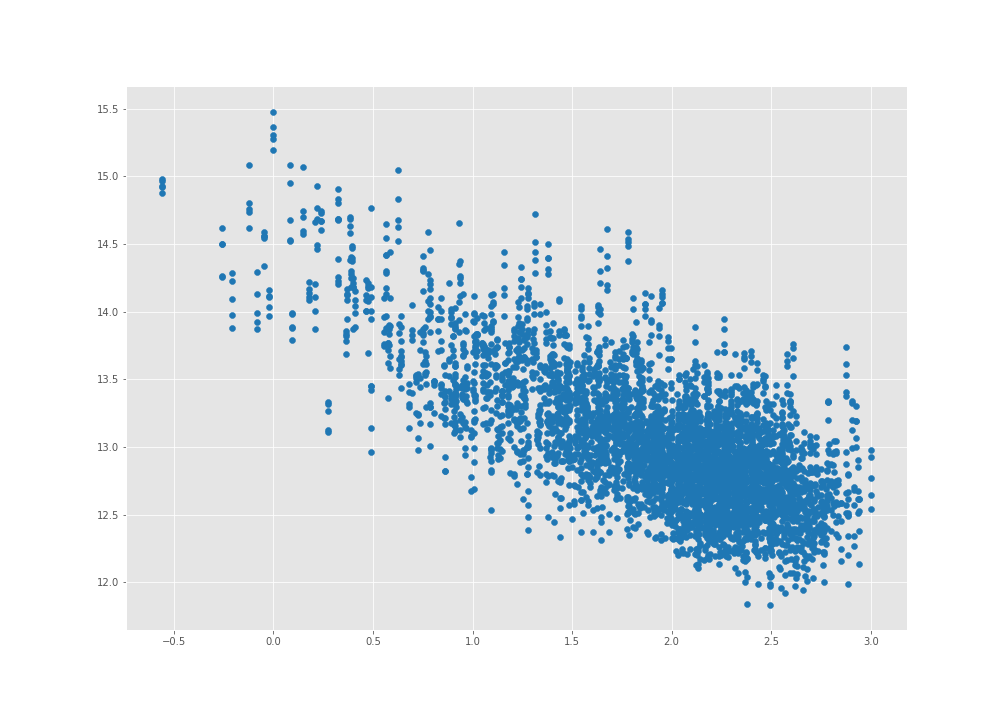
\includegraphics[width=\linewidth]{images/scatter_miles.png}
      \caption{log(Miles distance)}
      \label{fig:3(a)}
  \end{subfigure}
  \begin{subfigure}{.5\textwidth}
      \centering
      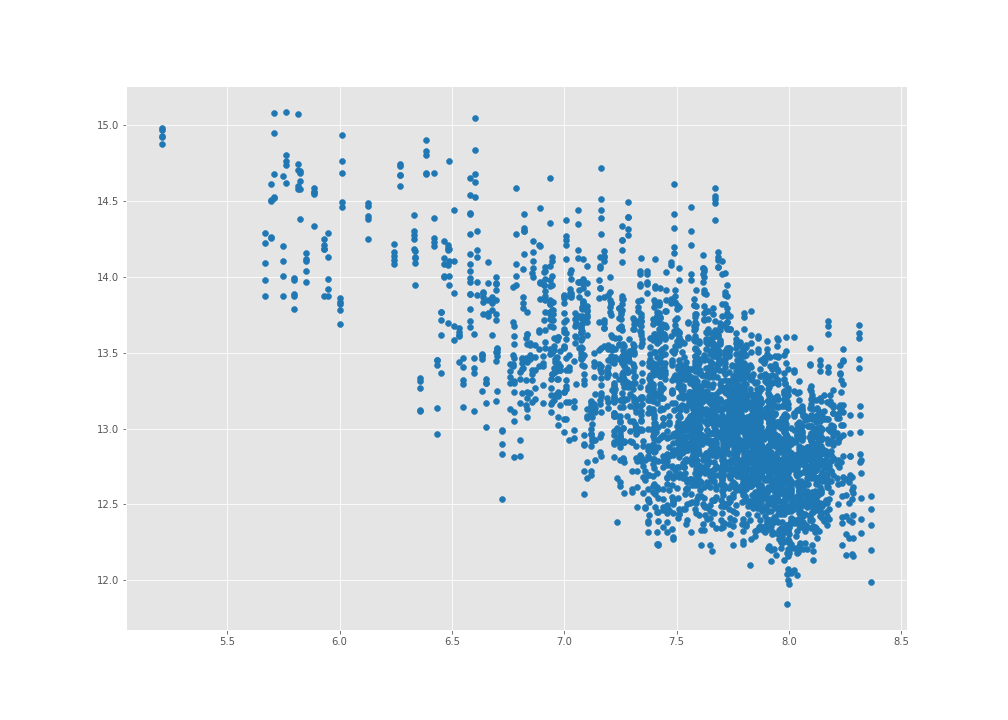
\includegraphics[width=\linewidth]{images/scatter_uber.png}
      \caption{log(Uber Distance in Average Minutes Travelled)}
      \label{fig:3(b)}
  \end{subfigure}
  \caption{Log-log Linearity Between Housing Price and Distance}
  \label{fig:log_log}
\end{figure}

\subsection{Geographical Features from OpenStreetMap}

\section{Empirical Analysis} \label{section:model}
\subsection{Model Specifications}
\subsection{Results}
\subsubsection{Monocentric City Model}
% monocentric city model
\begin{table}[H] \centering 
  \caption{Commuting cost estimate} 
  \label{} 
\small 
\begin{tabular}{@{\extracolsep{-10pt}}lcc} 
\\[-1.8ex]\hline 
\hline \\[-1.8ex] 
 & \multicolumn{2}{c}{\textit{Dependent variable:}} \\ 
\cline{2-3} 
\\[-1.8ex] & \multicolumn{2}{c}{log\_price} \\ 
\\[-1.8ex] & (1) & (2)\\ 
\hline \\[-1.8ex] 
 dist\_miles\_log & $-$0.584$^{***}$ &  \\ 
  & (0.021) &  \\ 
  & & \\ 
 uber\_dist\_mean\_log &  & $-$0.651$^{***}$ \\ 
  &  &                                                                                                                                                                   (0.025) \\ 
  & & \\ 
 Constant & 14.299$^{***}$ & 18.216$^{***}$ \\ 
  & (0.038) & (0.194) \\ 
  & & \\ 
\hline \\[-1.8ex] 
Observations & 726 & 726 \\ 
R$^{2}$ & 0.525 & 0.475 \\ 
Adjusted R$^{2}$ & 0.525 & 0.474 \\ 
\hline 
\hline \\[-1.8ex] 
\textit{Note:}  & \multicolumn{2}{r}{$^{*}$p$<$0.1; $^{**}$p$<$0.05; $^{***}$p$<$0.01} \\ 
\end{tabular} 
\end{table} 


\subsubsection{Hedonic Pricing Model}
% hedonic pricing model
\begin{table}[H] \centering 
  \caption{Cross-sectional OLS} 
  \label{} 
\small 
\begin{tabular}{@{\extracolsep{-10pt}}lcccccc} 
\\[-1.8ex]\hline 
\hline \\[-1.8ex] 
 & \multicolumn{6}{c}{\textit{Dependent variable:}} \\ 
\cline{2-7} 
\\[-1.8ex] & \multicolumn{6}{c}{log\_price} \\ 
\\[-1.8ex] & (1) & (2) & (3) & (4) & (5) & (6)\\ 
\hline \\[-1.8ex] 
 dist\_miles\_log & $-$0.513$^{***}$ & $-$0.491$^{***}$ & $-$0.478$^{***}$ & $-$0.464$^{***}$ & $-$0.463$^{***}$ & $-$0.438$^{***}$ \\ 
  & (0.015) & (0.015) & (0.015) & (0.015) & (0.015) & (0.015) \\ 
  & & & & & & \\ 
 supermarket\_high &  & 0.109$^{***}$ & 0.095$^{***}$ & 0.076$^{***}$ & 0.073$^{***}$ & 0.051$^{**}$ \\ 
  &  & (0.023) & (0.022) & (0.022) & (0.022) & (0.022) \\ 
  & & & & & & \\ 
 supermarket\_low &  & $-$0.157$^{***}$ & $-$0.130$^{***}$ & $-$0.113$^{***}$ & $-$0.112$^{***}$ & $-$0.109$^{***}$ \\ 
  &  & (0.030) & (0.028) & (0.028) & (0.028) & (0.027) \\ 
  & & & & & & \\ 
 residential &  &  & 0.008$^{***}$ & 0.009$^{***}$ & 0.009$^{***}$ & 0.008$^{***}$ \\ 
  &  &  & (0.002) & (0.002) & (0.002) & (0.002) \\ 
  & & & & & & \\ 
 retail &  &  & 0.0002 & 0.001 & 0.0004 & 0.0002 \\ 
  &  &  & (0.002) & (0.002) & (0.002) & (0.002) \\ 
  & & & & & & \\ 
 industrial &  &  & $-$0.031$^{***}$ & $-$0.026$^{***}$ & $-$0.026$^{***}$ & $-$0.024$^{***}$ \\ 
  &  &  & (0.005) & (0.005) & (0.005) & (0.005) \\ 
  & & & & & & \\ 
 construction &  &  & 0.011$^{**}$ & 0.006 & 0.006 & 0.006 \\ 
  &  &  & (0.005) & (0.005) & (0.005) & (0.005) \\ 
  & & & & & & \\ 
 commercial &  &  & 0.004 & $-$0.013$^{**}$ & $-$0.013$^{**}$ & $-$0.013$^{**}$ \\ 
  &  &  & (0.005) & (0.006) & (0.006) & (0.006) \\ 
  & & & & & & \\ 
%  garden &  &  & 0.0004 & 0.0003 & 0.0003 & 0.0004 \\ 
%   &  &  & (0.001) & (0.001) & (0.001) & (0.001) \\ 
%   & & & & & & \\ 
%  pitch &  &  & 0.006$^{***}$ & 0.005$^{***}$ & 0.005$^{***}$ & 0.003$^{***}$ \\ 
%   &  &  & (0.001) & (0.001) & (0.001) & (0.001) \\ 
%   & & & & & & \\ 
%  park &  &  & $-$0.003 & $-$0.003$^{*}$ & $-$0.003$^{*}$ & $-$0.003 \\ 
%   &  &  & (0.002) & (0.002) & (0.002) & (0.002) \\ 
%   & & & & & & \\ 
%  playground &  &  & $-$0.030$^{***}$ & $-$0.028$^{***}$ & $-$0.028$^{***}$ & $-$0.022$^{***}$ \\ 
%   &  &  & (0.006) & (0.006) & (0.006) & (0.006) \\ 
%   & & & & & & \\ 
%  nature\_reserve &  &  & 0.009 & 0.018 & 0.017 & 0.036 \\ 
%   &  &  & (0.028) & (0.027) & (0.027) & (0.026) \\ 
%   & & & & & & \\ 
 golf\_course &  &  & 0.198$^{***}$ & 0.185$^{***}$ & 0.179$^{***}$ & 0.147$^{***}$ \\ 
  &  &  & (0.035) & (0.034) & (0.034) & (0.033) \\ 
  & & & & & & \\ 
%  hotel &  &  &  & $-$0.002 & $-$0.002 & $-$0.002 \\ 
%   &  &  &  & (0.004) & (0.004) & (0.004) \\ 
%   & & & & & & \\ 
%  attraction &  &  &  & 0.016$^{*}$ & 0.016$^{*}$ & 0.020$^{**}$ \\ 
%   &  &  &  & (0.009) & (0.009) & (0.009) \\ 
%   & & & & & & \\ 
%  museum &  &  &  & 0.052$^{*}$ & 0.053$^{*}$ & 0.040 \\ 
%   &  &  &  & (0.029) & (0.029) & (0.028) \\ 
%   & & & & & & \\ 
%  art &  &  &  & 0.037 & 0.037 & 0.002 \\ 
%   &  &  &  & (0.024) & (0.024) & (0.023) \\ 
%   & & & & & & \\ 
 restaurant &  &  &  & 0.005$^{**}$ & 0.005$^{**}$ & 0.006$^{**}$ \\ 
  &  &  &  & (0.002) & (0.002) & (0.002) \\ 
  & & & & & & \\ 
 pub &  &  &  & 0.005 & 0.004 & 0.004 \\ 
  &  &  &  & (0.005) & (0.005) & (0.005) \\ 
  & & & & & & \\ 
 cafe &  &  &  & 0.005 & 0.006 & 0.004 \\ 
  &  &  &  & (0.006) & (0.006) & (0.005) \\ 
  & & & & & & \\ 
 fast\_food &  &  &  & $-$0.022$^{***}$ & $-$0.022$^{***}$ & $-$0.021$^{***}$ \\ 
  &  &  &  & (0.005) & (0.005) & (0.004) \\ 
  & & & & & & \\ 
 school &  &  &  &  & 0.011$^{**}$ &  \\ 
  &  &  &  &  & (0.005) &  \\ 
  & & & & & & \\ 
 private\_school &  &  &  &  &  & 0.120$^{***}$ \\ 
  &  &  &  &  &  & (0.014) \\ 
  & & & & & & \\ 
 university &  &  &  &  & 0.004 & 0.002 \\ 
  &  &  &  &  & (0.006) & (0.006) \\ 
  & & & & & & \\ 
 Constant & 14.330$^{***}$ & 14.280$^{***}$ & 14.230$^{***}$ & 14.200$^{***}$ & 14.180$^{***}$ & 14.130$^{***}$ \\ 
  & (0.035) & (0.036) & (0.037) & (0.038) & (0.040) & (0.038) \\ 
  & & & & & & \\ 
\hline \\[-1.8ex] 
Observations & 951 & 951 & 951 & 951 & 951 & 951 \\ 
R$^{2}$ & 0.543 & 0.565 & 0.635 & 0.654 & 0.656 & 0.680 \\ 
Adjusted R$^{2}$ & 0.543 & 0.563 & 0.629 & 0.646 & 0.647 & 0.672 \\ 
\hline 
\hline \\[-1.8ex] 
\textit{Note: Control variables include nature \& tourist amenities}  & \multicolumn{6}{r}{$^{*}$p$<$0.1; $^{**}$p$<$0.05; $^{***}$p$<$0.01} \\ 
\end{tabular} 
\end{table} 

\subsection{Causal Analysis of Supermarket Amenities}
retail area median (more than 5 multipolygons) \\
random oversampling \\
    => imbalanced dataset (correlation difficult to establish) \\
    
supermarket high (corr -0.4) \\
supermarket low (corr 0.7) \\

exclusion condition \\ 
    => corr resid -0.08 \\
    

\begin{table}[H] \centering 
  \caption{Instrumental Variables} 
  \label{} 
\begin{tabular}{@{\extracolsep{5pt}}lcc} 
\\[-1.8ex]\hline 
\hline \\[-1.8ex] 
 & \multicolumn{2}{c}{\textit{Dependent variable:}} \\ 
\cline{2-3} 
\\[-1.8ex] & \multicolumn{2}{c}{log\_price} \\ 
\\[-1.8ex] & \textit{OLS} & \textit{IV} \\
\\[-1.8ex] & (1) & (2)\\ 
\hline \\[-1.8ex] 
 dist\_miles\_log & $-$0.438$^{***}$ & $-$0.360$^{***}$ \\ 
  & (0.015) & (0.047) \\ 
  & & \\ 
supermarket\_high
  & 0.051$^{**}$ & 0.836$^{**}$ \\ 
  (Instrument: non-residential planning permits) & (0.022) & (0.384) \\ 
  & & \\ 
 supermarket\_low & $-$0.109$^{***}$ & $-$0.950$^{*}$ \\ 
  (Instrument: mean retail area) & (0.027) & (0.568) \\ 
  & & \\
%  residential & 0.008$^{***}$ & 0.007$^{**}$ \\ 
%   & (0.002) & (0.003) \\ 
%   & & \\ 
%  retail & 0.0002 & 0.003 \\ 
%   & (0.002) & (0.004) \\ 
%   & & \\ 
%  industrial & $-$0.024$^{***}$ & $-$0.016 \\ 
%   & (0.005) & (0.012) \\ 
%   & & \\ 
%  construction & 0.006 & $-$0.025 \\ 
%   & (0.005) & (0.018) \\ 
%   & & \\ 
%  commercial & $-$0.013$^{**}$ & 0.001 \\ 
%   & (0.006) & (0.013) \\ 
%   & & \\ 
%  garden & 0.0004 & $-$0.0003 \\ 
%   & (0.001) & (0.001) \\ 
%   & & \\ 
%  pitch & 0.003$^{***}$ & 0.007$^{**}$ \\ 
%   & (0.001) & (0.003) \\ 
%   & & \\ 
%  park & $-$0.003 & $-$0.007 \\ 
%   & (0.002) & (0.004) \\ 
%   & & \\ 
%  playground & $-$0.022$^{***}$ & $-$0.025$^{**}$ \\ 
%   & (0.006) & (0.011) \\ 
%   & & \\ 
%  nature\_reserve & 0.036 & 0.010 \\ 
%   & (0.026) & (0.050) \\ 
%   & & \\ 
 golf\_course & 0.147$^{***}$ & 0.089 \\ 
  & (0.033) & (0.070) \\ 
  & & \\ 
%  hotel & $-$0.002 & $-$0.002 \\ 
%   & (0.004) & (0.007) \\ 
%   & & \\ 
%  attraction & 0.020$^{**}$ & $-$0.010 \\ 
%   & (0.009) & (0.022) \\ 
%   & & \\ 
%  museum & 0.040 & 0.045 \\ 
%   & (0.028) & (0.051) \\ 
%   & & \\ 
%  art & 0.002 & $-$0.051 \\ 
%   & (0.023) & (0.050) \\ 
%   & & \\ 
 restaurant & 0.006$^{**}$ & 0.007 \\ 
  & (0.002) & (0.004) \\ 
  & & \\ 
 pub & 0.004 & $-$0.003 \\ 
  & (0.005) & (0.011) \\ 
  & & \\ 
 cafe & 0.004 & $-$0.009 \\ 
  & (0.005) & (0.013) \\ 
  & & \\ 
 fast\_food & $-$0.021$^{***}$ & $-$0.004 \\ 
  & (0.004) & (0.013) \\ 
  & & \\ 
 private\_school & 0.120$^{***}$ & 0.048 \\ 
  & (0.014) & (0.043) \\ 
  & & \\ 
 university & 0.002 & 0.011 \\ 
  & (0.006) & (0.013) \\ 
  & & \\
 Constant & 14.131$^{***}$ & 13.974$^{***}$ \\ 
  & (0.038) & (0.107) \\ 
  & & \\
 Controls: land use, nature \& tourist amenities & YES &   YES \\   &  &   \\ &  &  \\
\hline \\[-1.8ex] 
Weak instruments (supermarket\_high) &  & 0.000 \\ 
Weak instruments (supermarket\_low) &  & 0.001 \\ 
Wu-Hausman &  & 0.001  \\ 
Observations & 951 & 951 \\ 
R$^{2}$ & 0.680 & $-$0.070 \\ 
Adjusted R$^{2}$ & 0.672 & $-$0.097 \\ 
Residual Std. Error (df = 926) & 0.258 & 0.472 \\ 
\hline \\[-1.8ex]
\textit{Note: $R^{2} = 1- \frac{RSS}{TSS} < 0$ with endogeneity for IV}  & \multicolumn{2}{r}{$^{*}$p$<$0.1; $^{**}$p$<$0.05; $^{***}$p$<$0.01} \\ 
\end{tabular} 
\end{table} 
    
    
\section{Discussion} \label{section:discussion}

\subsection{External Validity}
\subsection{Limitations and Future Work}

\section{Conclusion} \label{section:conclusion}

\newpage
\nocite{*}
\renewcommand\harvardyearleft{\unskip, }
\renewcommand\harvardyearright[1]{.}
\let\oldthebibliography\thebibliography
\renewcommand\thebibliography{\let\bf\relax\oldthebibliography}
\renewcommand{\refname}{\textbf{Bibliography}}
\bibliographystyle{agsm}  
\bibliography{bibliography.bib}

\end{document}